%-------------------------------------------------------------------------
%-------------------------------------------------------------------------
% Modelo de TGR para o curso de Licenciatura em Matemática - UDESC/CCT
%
% Este modelo usa o pacote ABNTeX2, para instalar siga as seguintes instruções:
% Para poder usar o ABNTeX2 é necessário ter o LaTeX instalado. Para Windows, o MikTeX é o mais usado. 
% Vá até a página de download do abntex2 (http://code.google.com/p/abntex2/downloads/list), baixe uma das versões (eu usei abntex2.tds-1.7.1.zip) e descompacte em uma pasta temporária.
% Encontre a pasta na qual o MikTeX instalou seus arquivos (no meu computador foi C:\Arquivos de Programas(x86)\MikTex 2.9).
% Vá na pasta C:\temp\abntex-<versão>\texmf, selecione o conteúdo e copie tudo.
% Agora vá na pasta de instalação do MikTex e cole tudo (talvez vá sobrescrever alguma coisa). São os diretórios bibtex, doc e tex.
% Feito isso, será necessário atualizar o MikTeX destas mudanças. Para isso, vá em  Iniciar/Programas/MikTeX/Maintenance(Admin)/Settings e clique no botão Refresh Now.
% No Linux basta instalar o pacote texlive-full.
%
%
% ------------------------------------------------------------------------
% ------------------------------------------------------------------------

\documentclass[
	% -- opções da classe memoir --
	12pt,				% tamanho da fonte
	oneside,			% para impressão em verso e anverso. Oposto a oneside
	a4paper,			% tamanho do papel. 
	% -- opções do pacote babel --
	english,			% idioma adicional para hifenização
	french,				% idioma adicional para hifenização
	spanish,			% idioma adicional para hifenização
	brazil,				% o último idioma é o principal do documento
	]{abntex2}


% ---
% PACOTES
% ---

% ---
% Pacotes fundamentais 
% ---
\usepackage{cmap}				% Mapear caracteres especiais no PDF
\usepackage{
lmodern}			% Usa a fonte Latin Modern			
\usepackage[T1]{fontenc}		% Selecao de codigos de fonte.
\usepackage[utf8]{inputenc}		% Codificacao do documento (conversão automática dos acentos)
\usepackage{lastpage}			% Usado pela Ficha catalográfica
\usepackage{indentfirst}		% Indenta o primeiro parágrafo de cada seção.
\usepackage{color}				% Controle das cores
%\usepackage[dvips]{graphicx}    % Inclusão de gráficos (.eps)
\usepackage{graphicx} 
\usepackage{epstopdf}			%conversão direta para pdf permitindo inserir figuras jpg
\usepackage{amsmath}
\usepackage{amsfonts}
\usepackage{amssymb}
\usepackage{amsthm}
\usepackage[left=3cm,right=2cm,top=3cm,bottom=2cm]{geometry}


% ---
\usepackage{titlesec} %Adequação dos títulos as normas da UDESC
% ---
\titleformat{\chapter}
{\normalfont\normalfont\bfseries}
{\thechapter.}{0.5em}{}



\titleformat{\section}
{\normalfont}
{\thesection.}{0.5em}{}

\titleformat{\subsection}
{\normalfont}
{\thesection.}{0.5em}{}

% ---
\usepackage{etoc} %Adequação do sumário as normas da UDESC
% ---

\etocsetstyle{section}
{\normalfont}
{\addvspace{.5ex}\noindent\setlength{\leftskip}{1.5cm}\noindent}
{\llap{\makebox[1.5cm][l]{{\etocnumber}}}\etocname
  \hspace{10pt}\nobreak\dotfill\hspace{10pt}{\etocpage}\par}
{}
\etocsetstyle{chapter} 
{\bfseries}
{\addvspace{.5ex}\setlength{\leftskip}{1.5cm}\noindent}
{\llap{\makebox[1.5cm][l]{\bfseries\etocnumber}}\etocname
  \hspace{10pt}\nobreak\dotfill\hspace{10pt}\etocpage\par}
{}

\etocsetstyle{chapter} 
{\bfseries}
{\addvspace{.5ex}\setlength{\leftskip}{1.5cm}\noindent}
{\llap{\makebox[1.5cm][l]{\bfseries\etocnumber}}\etocname
  \hspace{10pt}\nobreak\dotfill\hspace{10pt}\etocpage\par}
{}

\etocsetstyle{subsection}
{\bfseries}
{\addvspace{.5ex}\noindent\setlength{\leftskip}{1.5cm}\noindent}
{\llap{\makebox[1.5cm][l]{{\bfseries\etocnumber}}}\etocname
  \hspace{10pt}\nobreak\dotfill\hspace{10pt}{\etocpage}\par}
{}
\etocsetstyle{chapter} 
{\bfseries}
{\addvspace{.5ex}\setlength{\leftskip}{1.5cm}\noindent}
{\llap{\makebox[1.5cm][l]{\bfseries\etocnumber}}\etocname
  \hspace{10pt}\nobreak\dotfill\hspace{10pt}\etocpage\par}
{}

\etocsettocstyle{\chapter*{\bfseries SUMÁRIO}}
{\bfseries}
\setcounter{tocdepth}{1}
\setcounter{secnumdepth}{2}



% ---
% Novos Comandos 
% ---
\newcommand{\R}{\ensuremath {\mathbb{R}} }
\newcommand{\Z}{\ensuremath {\mathbb{Z}} }
\newcommand{\Q}{\ensuremath {\mathbb{Q}} }
\newcommand{\N}{\ensuremath {\mathbb{N}} }
\newcommand{\C}{\ensuremath {\mathbb{C}} }
\newcommand{\K}{\ensuremath {\mathbb{K}} }


% ---
% Estilo teoremas  e atalhos para comandos 
% ---
\theoremstyle{plain}
\newtheorem{teo}{Teorema}[chapter]
\newtheorem{prop}{Proposição}[chapter]
\newtheorem{lema}{Lema}[chapter]
\newtheorem{corol}{Corolário}[chapter]
\newtheorem{defi}{Definição}[chapter]

\theoremstyle{definition}
\newtheorem{obs}{Observação}[chapter]
\newtheorem{ex}{Exemplo}[chapter]

\newenvironment{dem}[1][\textbf{Demonstração:} \ ]{\textbf{#1}}{\hfill\rule{2mm}{2mm}}
\newcommand{\afi}{\textbf{Afirmação:} }
% ---

%\usepackage{lipsum}				% para geração de dummy text

% ---
% Pacotes de citações
% ---
\usepackage[brazilian,hyperpageref]{backref}	 % Paginas com as citações na bibl
\usepackage[alf]{abntex2cite}	% Citações padrão ABNT





% --- 
% CONFIGURAÇÕES DE PACOTES
% --- 

% ---
% Configurações do pacote backref
% Usado sem a opção hyperpageref de backref
\renewcommand{\backrefpagesname}{Citado na(s) página(s):~}
% Texto padrão antes do número das páginas
\renewcommand{\backref}{}
% Define os textos da citação
\renewcommand*{\backrefalt}[4]{
	\ifcase #1 %
		Nenhuma citação no texto.%
	\or
		Citado na página #2.%
	\else
		Citado #1 vezes nas páginas #2.%
	\fi}%
% ---

% ---
%%Cabeçalho
% ---
\makepagestyle{meuestilo}
  %%cabeçalhos
 % \makeevenhead{meuestilo} %%pagina par
   %  {topo par à esquerda}
   %  {centro \thepage}
    % {direita}
  \makeoddhead{meuestilo} %%pagina ímpar ou com oneside
     {} %esquerda
     {} %centro
     {\thepage}%direita
  
 

% ----
% Início
% ----

\titulo{TÍTULO: SUBTÍTULO (se houver)}
\autor{NOME DO AUTOR}
\local{JOINVILLE, SC}
\date{ANO}
\tipotrabalho{TRABALHO DE CONCLUSÃO DE CURSO}
\preambulo{ Trabalho de conclusão de curso apresentado como requisito parcial para obtenção do título de licenciado em Matemática pelo curso de Licenciatura em Matemática do Centro de Ciências Tecnológicas - CCT, da Universidade do Estado de Santa Catarina - UDESC. \\
 Orientador: Titulação + nome completo}
% ---


\makeatother
% --- 

% --- 
% Espaçamentos entre linhas e parágrafos 
% --- 

% O tamanho do parágrafo é dado por:
\setlength{\parindent}{1.25cm}

% Controle do espaçamento entre um parágrafo e outro:
\setlength{\parskip}{0.2cm}  % tente também \onelineskip

% ---
% compila o indice
% ---
\makeindex
% ---

% ----
% Início do documento
% ----
\begin{document}

% Retira espaço extra obsoleto entre as frases.
\frenchspacing 

% ----------------------------------------------------------
% ELEMENTOS PRÉ-TEXTUAIS
% ----------------------------------------------------------

\pretextual

% ---------------------------------------------
% capa
% ---------------------------------------------
\begin{center}
\thispagestyle{empty}%página não enumerada
 \textbf{ UNIVERSIDADE DO ESTADO DE SANTA CATARINA - UDESC\\
CENTRO DE CIÊNCIAS TECNOLÓGICAS - CCT\\
CURSO DE LICENCIATURA EM MATEMÁTICA\\}
\vspace{4 cm}\textbf{NOME DO AUTOR}

\vspace{4 cm}\textbf{TÍTULO DO TRABALHO:} SUBTÍTULO

\vspace{\stretch{1}}
\textbf{JOINVILLE - SC}

\textbf{2020}
 \pagebreak
\end{center}
% ---


% ------------------------------------------------
% folha de rosto
% ------------------------------------------------

\begin{folhaderosto}

  \begin{center}
    \textbf{NOME DO AUTOR}

    \vspace*{\fill}\vspace*{\fill}
    \textbf{TÍTULO DO TRABALHO:} SUBTÍTULO
    \vspace*{\fill}
  \end{center}
  
  \begin{flushright}
  \begin{minipage}[t]{8 cm}
  { Trabalho de conclusão de curso apresentado como requisito parcial para obtenção do título de licenciado em Matemática pelo curso de Licenciatura em Matemática do Centro de Ciências Tecnológicas - CCT, da Universidade do Estado de Santa Catarina - UDESC. 

 Orientador: Titulação + nome completo}
  \end{minipage}
  \end{flushright}
  
  \vspace{\stretch{1}}
  
  \begin{center}
 \textbf{JOINVILLE - SC}
 
 \textbf{2020} 
  \end{center}
\end{folhaderosto}
% ---



% ----------------------------------------------------
% Inserir folha de aprovação
% ----------------------------------------------------

% Isto é um exemplo de Folha de aprovação, elemento obrigatório da NBR
% 14724/2011 (seção 4.2.1.3). Você pode utilizar este modelo até a aprovação
% do trabalho. Após isso, substitua todo o conteúdo deste arquivo por uma
% imagem da página assinada pela banca com o comando abaixo:
%
% \includepdf{folhadeaprovacao_final.pdf}
% ---


% ---------------------------------------------------
% folha de aprovação
% ---------------------------------------------------
\begin{folhadeaprovacao}

  \begin{center}
    \textbf{NOME DO AUTOR}
\vspace {1 cm}

     \textbf{TÍTULO DO TRABALHO:} SUBTÍTULO
   \vspace {1 cm}
  \end{center}
    
\begin{flushright}
  \begin{minipage}[t]{8 cm}
  { Trabalho de conclusão de curso apresentado como requisito parcial para obtenção do título de licenciado em Matemática pelo curso de Licenciatura em Matemática do Centro de Ciências Tecnológicas - CCT, da Universidade do Estado de Santa Catarina - UDESC. 

 Orientador: Titulação + nome completo}
 
  \end{minipage}
  \end{flushright}
     
     \begin{minipage}[c]{3cm} 
	Membros:
\end{minipage}
\begin{minipage}[c]{8 cm}
	\begin{center}
	\textbf{BANCA EXAMINADORA}
	\vspace {2 cm}
	
	Nome do Orientador e Titulação
	
    Nome da Instituição
    
    \vspace {1.5 cm}
    
    Nome do Membro da banca e Titulação
	
    Nome da Instituição
    
    \vspace {1.5 cm}
    
    Nome do Membro da banca e Titulação
	
    Nome da Instituição
    \vspace {1.5 cm}
    
    
\end{center}

\end{minipage}

\vspace*{\fill}
     \begin{center}
	     Joinville, dia do mês e ano.
\end{center}

    
\end{folhadeaprovacao}
% ---



% ---------------------------------------
% Dedicatória
% ---------------------------------------
\vspace*{\fill}

\begin{dedicatoria}
   \vspace*{10 cm}
   \begin{flushright}
   \begin{minipage}[t]{7cm}
     Elemento opcional utilizado pelo autor para registrar homenagens ou dedicatórias à determinada(s) pessoa(s).
   \end{minipage}
   \end{flushright}
\end{dedicatoria}
% ---


% ---------------------------------------
% Agradecimentos
% ---------------------------------------
\begin{center}
	\textbf{AGRADECIMENTOS}
\end{center}

Elemento opcional utilizado pelo autor para registrar agradecimento às pessoas que contribuíram para a elaboração do trabalho.


\newpage
% ---


% -----------------------------------------
% Epígrafe
% -----------------------------------------
\vspace*{\fill}

\begin{epigrafe}
    \vspace*{10cm}
	\begin{flushright}
	  \begin{minipage}[t]{7cm}
		\textit{Elemento opcional utilizado pelo autor para apresentar uma citação relacionada com a matéria tratada no corpo do trabalho.}
		
	 \end{minipage}
	\end{flushright}
\end{epigrafe}
% ---


% -----------------------------------------
% RESUMOS
% -----------------------------------------
% resumo em português
\begin{center}
	\textbf{RESUMO}
\end{center}



  \vspace{\onelineskip}

\noindent Elemento obrigatório que contém a apresentação concisa dos pontos relevantes do trabalho, fornecendo uma visão rápida e clara do conteúdo e das conclusões do mesmo. A apresentação e a redação do resumo devem seguir os requisitos estipulados pela NBR 6028 (ABNT, 2003). Deve descrever de forma clara e sintética a natureza do trabalho, o objetivo, o método, os resultados e as conclusões, visando fornecer elementos para o leitor decidir sobre a consulta do trabalho no todo.

 \vspace{\onelineskip}
    
 \noindent\textbf{Palavras-chave:} Palavra 1. Palavra 2. Palavra 3. Palavra 4. Palavra 5.

\newpage


% resumo em inglês
 \begin{otherlanguage*}{english}

\begin{center}
	\textbf{ABSTRACT}
\end{center}



 \vspace{\onelineskip}

\noindent Elemento obrigatório para todos os trabalhos de conclusão de curso. Opcional para os demais trabalhos acadêmicos, inclusive para artigo científico. Constitui a versão do resumo em português para um idioma de divulgação internacional. Deve aparecer em página distinta e seguindo a mesma formatação do resumo em português.
 \vspace{\onelineskip}

\noindent\textbf{Keywords:} Keyword 1. Keyword 2. Keyword 3. Keyword 4. Keyword 5.

 \end{otherlanguage*}

\newpage


% ---


% -----------------------------------------
% inserir lista de ilustrações
% -----------------------------------------
\renewcommand\listfigurename{{\fontsize{12pt}{\baselineskip}\normalfont \bfseries LISTA DE ILUSTRAÇÕES}}
\pdfbookmark[0]{\listfigurename}{lof}
\listoffigures*
\cleardoublepage
% ---


% -----------------------------------------
% inserir lista de tabelas
% -----------------------------------------
\renewcommand\listtablename{{\fontsize{12pt}{\baselineskip}\normalfont \bfseries LISTA DE TABELAS}}
\pdfbookmark[0]{\listtablename}{lot}
\listoftables*
\cleardoublepage
% ---



% ----------------------------------------
% inserir lista de abreviaturas e siglas
% ----------------------------------------
\renewcommand\listadesiglasname{{\fontsize{12pt}{\baselineskip}\normalfont \bfseries LISTA DE ABREVIATURAS E SIGLAS}}
\begin{siglas}
  \item[ABNT]  Associação Brasileira de Normas Técnicas 
  \item[ENEM]  Exame nacional do Ensino Médio
  \item[Fig.]  Area of the $i^{th}$ component
  \item[FLT]   Fermat's Last Theorem  
  \item[MEC]   Ministério da Educação
  \end{siglas}
% ---


% ----------------------------------------
% inserir lista de símbolos
% ----------------------------------------
\renewcommand\listadesimbolosname{{\fontsize{12pt}{\baselineskip}\normalfont \bfseries LISTA DE SÍMBOLOS}}
\begin{simbolos}
  \item[$ \mathbb{N} $] Conjunto dos números naturais 
  \item[$ \mathbb{Z} $] Conjunto dos números inteiros 
  \item[$ \mathbb{Q} $] Conjunto dos números racionais 
  \item[$ \mathbb{R} $] Conjunto dos números reais 
  \item[$ \mathbb{C} $] Conjunto dos números complexos
  \item[$ C_c(R) $] Conjunto das funções $f: R \rightarrow \C$ contínuas com suporte compacto em um conjunto $R$.
\end{simbolos}
% ---


% ----------------------------------------
% inserir o sumario
% ----------------------------------------
\renewcommand\contentsname{{\fontsize{12pt}{\baselineskip}\normalfont \bfseries SUMÁRIO}}
\pdfbookmark[0]{\contentsname}{toc}
\tableofcontents*
\cleardoublepage
% ---



% ----------------------------------------------------------
% ELEMENTOS TEXTUAIS
% ----------------------------------------------------------

\textual

% ----------------------------------------------------------
% Introdução
% ----------------------------------------------------------
  \pagestyle{meuestilo}

\chapter{INTRODUÇÃO} % LETRAS MAIÚSCULAS


A introdução apresenta os objetivos do trabalho, bem como as razões de sua elaboração. Tem caráter didático de apresentação.
Deve abordar:

    a) o problema de pesquisa, proposto de forma clara e objetiva;
    
    b) os objetivos, delimitando o que se pretende fazer;
    
    c) a justificativa, destacando a importância do estudo;
    
    d) apresentar as definições e conceitos necessários para a compreensão do estudo;
    
    e) apresentar a forma como está estruturado o trabalho e o que contém cada uma de suas partes.
    
O desenvolvimento é a demonstração lógica de todo o trabalho, detalha a pesquisa ou o estudo realizado. Explica, discute e demonstra a pertinência das teorias utilizadas na exposição e resolução do problema. 

O desenvolvimento pode ser subdivido em seções e subseções com nomenclaturas definidas pelo autor conforme conteúdo apresentado. 
% ---



% ---------------------------------------------------------
% primeiro capítulo
% ---------------------------------------------------------
\chapter{CAPÍTULO FORMATO E FONTES} % LETRAS MAIÚSCULAS

Você deve sempre mudar de pagina ao iniciar um novo capitulo de seu trabalho.

Para os títulos utilizar o mesmo tipo e tamanho de fonte do texto. 

Usar fonte do tipo Arial ou Times New Roman com tamanho 12, espaçamento entre as linhas 1,5 cm, margem direta 2 cm, margem esquerda 3,0 cm, margem superior 3 cm e inferior com 2cm.

Citações com mais de três linhas, legendas de ilustrações e tabelas, rodapés devem ser digitados em tamanho 10 pt. Citações com mais de 3 linhas devem ter recuo de 4 cm a partir da esquerda.

Abaixo um exemplo de como citar a bibliografia no texto

\begin{citacao}
 Tal disciplina é caracterizada pelo estudo de funções reais ligadas aos processos de limite e pelo fato de seu conteúdo apoiar-se sobre quase todo o saber escolar ensinado aos alunos até então (BARROSO et al, 2009, p.).
\end{citacao}

Para as divisões principais utilizar maiúsculo e negrito, divisão secundária em letras maiúsculas sem negrito, seção terciária fonte normal com as primeiras letras em maiúsculo e em negrito, seção quartenária utilizar fonte normal somente a primeira letra da primeira palavra em maiúsculo, conforme ex.

%---

% ---
\section{EXEMPLOS} % LETRAS MAIÚSCULAS
% ---


Nesta seção veremos alguns exemplos de teorema, proposição, observação, lema, formas de numeração, equações, etc.  O texto a seguir não faz muito sentido, são pequenas partes tiradas da minha dissertação de mestrado.

\begin{defi}
Uma álgebra é um espaço vetorial $A$ sobre o corpo dos números complexo $\C$, munida com uma multiplicação que satisfaz:
\begin{itemize}
\item $a(bc)=(ab)c$
\item $(a+b)c = ac+bc$, \,\,\, $a(b+c)=ab+ac$
\item $\lambda(ab)=(\lambda a)b=a(\lambda b)$
\end{itemize}
para quaisquer $a, b, c \in A$ e $\lambda \in \C.$
\end{defi}

\begin{obs}
Se $A$ é um espaço de Banach com relação a uma norma, $\Vert \cdot \Vert $, tal que $$\Vert ab \Vert \leq \Vert a \Vert \Vert b \Vert$$ para quaisquer $a, b \in A$, então $A$ é uma álgebra de Banach.
\end{obs}


\begin{defi} 
Uma involução em uma álgebra $A$ é uma aplicação $\ast: A \rightarrow A$ que satisfaz:
\begin{enumerate}
\item $(a+b)^{\ast}= a^{\ast}+b^{\ast}$
\item $(\lambda a )^{\ast} = \overline{\lambda} a^{\ast}$
\item $(ab)^{\ast}=b^{\ast}a^{\ast}$
\item ${a^{\ast}}^{\ast}=a$
\end{enumerate}
para quaisquer $a, b \in A$ e $\lambda \in \C.$ Uma álgebra $A$ munida de uma involução é chamada de $\ast$ - álgebra.
\end{defi}
% ---


Abaixo um exemplo de como citar a bibliografia no texto.

O exemplo do corpo quadrático $\Q[\sqrt{-5}]$ mostra que o anel dos inteiros algébrico de um corpo de número algébricos nem sempre  fatorial.  De acordo com \cite{endler2006}, para consertar esta falha, foi introduzido por Kummer a noção de "número ideal", que deu origem à noção de "ideal" devida a Dedekind.


% ---
\subsection{Mais exemplos} %Letras Maiúsculas e Minículas
% ---


\begin{defi}\
\begin{enumerate}
\renewcommand{\labelenumi}{(\alph{enumi})} % numeração (a), (b), (c) ...
\item  seminorma sobre um espaço vetorial $X$ é uma função $p: X \rightarrow \R_{+}$ tal que
\begin{description}
\item[$\star$] $p(x+y)\leq p(x)+p(y)$
\item[$\star$] $p(\lambda x)= |\lambda|p(x)$
\end{description}
para todo $x, y \in X$ e $\lambda \in \C$. \\
\item  Uma C*-seminorma $p$ sobre uma $\ast$ -álgebra $A$ é uma seminorma que satisfaz, para todo $x, y \in A$,
\begin{description}
\item[$\diamond$] $p(xy)\leq p(x)p(y)$
\item[$\diamond$] $p(x^*)=p(x)$
\item[$\diamond$] $p(x^*x)=p(x)^2.$
\end{description}
\end{enumerate}
\end{defi}


\begin{lema} 
Seja $G$ um grupóide.
\renewcommand{\labelenumi}{(\roman{enumi})} % numeração (i), (ii), ...
\begin{enumerate}
  \item $G^0 = \{x \in G \,\, : \,\, x=x^{-1}\}$.
  \item $G^2=\{(x,y) \in G \times G \,\, : \,\, s(x)=r(y)\}$.
\end{enumerate}
\end{lema}


\noindent \begin{dem} 
Se $x \in G^0$ então existe $y \in G$ tal que $x=yy^{-1}$, logo $x^{-1}=(yy^{-1})^{-1}= yy^{-1}=x$. 
\par $(\supseteq)$ Seja $x \in G$ tal que $x=x^{-1}$. Suponha que não existe $y \in G$ tal que $x=yy^{-1}$, ou seja, $x \neq yy^{-1}$ para todo $y \in G$. Então $x^{-1} \neq (yy^{-1})^{-1}=yy^{-1}=x$, implica que $x^{-1}\neq x$. Absurdo! Portanto existe $y \in G$ tal que $x=yy^{-1}$ e $x \in G^0$...
\end{dem}


Equações:

\begin{equation}\label{produto}  
f \ast g (x,z) = \sum_{y \in [x]} f(x,y)g(y,z),
\end{equation}

\begin{equation}\label{involucao} 
f^*(x,y)= \overline{f(x,y)}.
\end{equation}


\begin{prop}\label{continuas}
Seja $R$ uma relação étale então as aplicações range e source são contínuas.
\end{prop}


\begin{obs} 
Pela Proposição \ref{continuas}, temos que $r$ é uma aplicação contínua, então $r|_{\bigtriangleup}$ também é uma aplicação contínua. Portanto $\bigtriangleup = \left(r|_{\bigtriangleup}\right) ^{-1}(X)$ é aberta em $(R, \tau)$.
\end{obs}


Da equação \ref{involucao}, segue que
\begin{align*}  
        X & = \sum_{z \in [y]}\overline{f(y,z)}\,\overline{g(z,x)}= \sum_{z \in [y]} f^*(z,y)g^*(x,z)\\
          & = \sum_{z\in [y]}g^*(x,z)f^*(z,y) = g^* \ast f^* (x,y)
\end{align*}


\begin{teo}
Para uma relação étale $R$ e  $x \in X$ a representação  $\lambda_x$ definida acima é uma representação não-degenerada e limitada de $C_c(R)$.
\end{teo}




% ----------------------------------------------------------
% segundo capítulo
% ----------------------------------------------------------
\chapter{FIGURAS E TABELAS}

Exemplos de inserção de figura e tabela.

% ---
\section{INSERIR FIGURAS}
% ---

As identificações de qualquer tipo de ilustração devem aparecer na parte superior, precedida da palavra designativa, seguida de seu número de ordem de ocorrência no texto, em algarismos arábicos, travessão e do respectivo título (texto com espaçamento entrelinhas simples e fonte 12). Na parte inferior deve-se indicar a fonte consultada (tamanho 10). Todas as figuras devem ser centralizadas em relação a margem. A figura deve ser colocada após sua citação no texto, deixando-se entrelinhas 1,5 entre o texto e a figura. Após a figura, o texto segue a um espaço de 1,5. Veja na Figura 1 um exemplo de figura:

Seguem dois exemplos de figuras:

Aqui a figura fica dentro de um retângulo (caixa).

\begin{figure}[!h]
	\centering  
	\caption{Diagrama de Bratteli}
	\label{diagrama}
	\fbox{
\includegraphics[width=10cm,height=8cm]{diagrama.eps}}
	\fonte{{\small Produção do autor}}    
\end{figure}

Fora da caixa.

\begin{figure*}[!h]
	\centering
	\caption{Título da Figura}
	\label{referencia}
	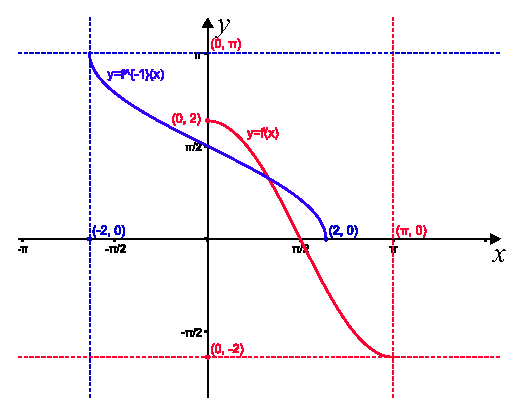
\includegraphics[width=7cm]{exemplo1.eps}
	\fonte{{\small Produção do autor}}
\end{figure*}




%---------
\section{CRIAR TABELA}

Segundo a ABNT em tabelas não deve-se utilizar linhas verticais para separar as colunas, conforme exemplo abaixo na Tabela \ref{tabelaABNT}. 

\begin{table}[!h]
	\centering
	\caption{Percentual de alunos aprovados e reprovados na disciplina de Cálculo I por curso}
	\label{tabelaABNT}
	\begin{tabular}{l c c} \hline
		\textbf{Curso}   &   \textbf{Aprovados (\%)}   &   \textbf{Reprovados (\%)}  \\  \hline
		Engenharia Civil   &  65  &  35   \\   
		Engenharia Elétrica &  40  &  60   \\ 
		Engenharia Mecânica   & 68 & 32 \\
		Engenharia de Produção & 34 &  66\\ \hline
	\end{tabular}
	\fonte{{\small Acervo do autor}}
	
\end{table}






% ------------------------------------------------------------
% Conclusão
% ------------------------------------------------------------
\chapter*[Conclusão]{CONSIDERAÇÕES FINAIS}
\addcontentsline{toc}{chapter}{CONSIDERAÇÕES FINAIS}

É a parte final do texto. Deve retomar o problema inicial, revendo os objetivos
e comentando se foram atingidos ou não, enunciando as principais contribuições.
Sintetiza as principais idéias, bem como os resultados, avaliando pontos positivos e
negativos. Geralmente inclui recomendações e/ou sugestões. 

% ----------------------------------------------------------
% Referências bibliográficas
% ----------------------------------------------------------
	\chapter*[Referências]{REFERÊNCIAS}
\addcontentsline{toc}{chapter}{REFERÊNCIAS}




%\bibliography{bibliografia}





% ----------------------------------------------------------
% Apêndices
% ----------------------------------------------------------


\chapter*[Apêndice]{APÊNDICE A - TÍTULO}
\addcontentsline{toc}{chapter}{APÊNDICE A - TÍTULO}
% ----------------------------------------------------------

Lalalalalala....

% ----------------------------------------------------------
%\chapter{Titulo do Segundo Apêndice}
% ----------------------------------------------------------

%Lalalalalala...


% ---


% ----------------------------------------------------------
% Anexos
% ----------------------------------------------------------



% ---
\chapter*[Anexos]{ANEXO A - TÍTULO}
\addcontentsline{toc}{chapter}{ANEXO A - TÍTULO}
% ---

Lalalalalala...

% ---
%\chapter{Nome do anexo 2}
% ---

%lalalalalalalala....



%---------------------------------------------------------------------
% INDICE REMISSIVO
%---------------------------------------------------------------------

\printindex

\end{document}
